\subsection{Android}
Comme nous l'avons mentionné dans les rubriques précédentes, le client à été developpé pour Android. Pour cela, nous avons choisi d'utiliser le langage Kotlin qui est plus preformant et optimise les opérations et la structure en opposition à Java. C'est également le langage que nous utilisons au sein du cours d'Android, c'est donc un bon moyen de mettre en relation les deux cours.

Le rôle principal de ce client est de détecter (grâce au bluetooth) le beacoin avec la plus grande proximité. En fonction de ce beacoin le client peut envoyer une requête permettant de determiner la salle dans laquel se trouve la personne et les devices qui y ont présentes (stors, radiateurs, lumières etc.).Une fois l'emplacement determiné et les devices détéctés, les contrôles et les informations des différents devies apparaissent sur l'interface graphique de l'utilisateur, lui permettant de contrôller ou obtenir les différentes informations des devices à proximité. 

\subsection{Broker Kafka}
Le broker Kafka joue le rôle de coordinateur entre tous les différents clients qui consomment et produisent des messages dans les différents topics.
Nous avons choisi de déployer ce Broker Kafka sur une instance AWS permettant de le rendre accessible par toutes les entités de l'application.
Nous avons également associé un nom de domaine à cette instace ce qui permet de la référencer de manière plus lisible et agérable par les clients.

\subsection{Rest server Flask}
Etant donné qu'il n'existe pas enciore de librairie permettant d'utiliser dirctement le client Kafka sur Android, nous avons du mettre en place un adapter que nous permet de faire la translation entre Kafka Android.
Pour ce faire nous avons utilisé la librairie Flask de Python 3 qui permet de mettre en place une API REST.
Cette API joue également le rôle de producteur et de consumateur Kafka afin de mettre en relation les différentes entités.
D'une part, le consomateur Kafka se charge de consommer les différents messages de KNX et Openzwave afin de stocker les informations utiles à l'application et aux statistiques dans la base de données.
D'autre part, nous avons le producteur Kafka qui se charge de transformer les actions reçues sous forme de requête HTTP en message Kafka envoyé directement dans le bon topic ce qui permet donc d'effectuer les actions demandées en conséquence (ouverture des stors par exemple).

\subsubsection{Routes exposées}
Voici la liste exhaustive des différentes routes mise à disposition par notre API REST : 
% TODO: prendre les routes et bien formatter


\subsection{KNX lib}
En se basant sur le code de l'exercice KNX réalisé au cours du premier service, nous l'avons adapté de manière à en faire une librairie réutilisabe depuis les producteur et consomateur Kafka.
Cette libraire contient une classe \mintinline{python}{knx} qui se charge de créer la connexion avec knx dans son constructeur et expose les différentes méthodes relatives à l'utilisation des devies KNX.
Voici les méthodes intégrées à notre libraire KNX :
\begin{itemize}
    \item \mintinline{python}{send_datas(self, group_address, data, data_size, apci, read=False)} : cette méthode est utilisée afin de transmettre des informations à KNX elle recoit différents arguments variables qui permettent de controller/lire les informations des différentes devices en adaptant leurs emplacement qui sont identifiable à l'aide de l'étage et de la salle (voir protocole KNX).
    \item \mintinline{python}{disconnect(self)} => permet de se deconnecter de KNX
\end{itemize}

\subsection{Zwave lib}
Nous avons réutilisé la librairie que nous avions développée durant le premier semestre qui comprend les différentes méthodes permettnt d'intéragir avec le réseau Openzwave. 
Dans le cadre de ce projet, nous n'utilisons plus cette libraire au travers d'un serveur Flask, mais directemnt dans le producteur et le consommateur Kafka.
Tout cela nous permet donc d'appliquer différentes actions qui ont été consummée et également de produire à intervalles réguliers les informations émise par les devices de notre salle.

% TODO: revoir
\subsection{Adapter Kafka OUUU ?????? Protocole des messages}
En ce qui concerne les messages consommés par KNX et openzwave, nous avons choisi de définir notre propre protocol.
Celui ci fait correspondre la clé du message reçu à l'action à effectuer et le contenu du message aux éventuels paramètres à transmettre. Ces différents paramètres sont au format JSON puis encodés en bytes afin d'être transmits au broker Kafka consumés par une autre entité.

\subsubsection{KNX}
Pour KNX nous retrouvons les messages suivants : 
\paragraph{Production}
\begin{itemize}
    \item \mintinline{python}{read_percentage_blinds} : Ce messages est produit à intervalles de 5 secondes, il permet d'envoyer dans le topic \mintinline{text}{KNX} le pourcentage d'ouverture de tous les stores de toutes les salles. 
\end{itemize}

\paragraph{Consommation}
    L'étage et la chambre permettent d'identifier l'appareil sur lequel il faut agir, pour cela ces deux paramètres sont donnés dans le corps du message ce qui permet d'intéragir avec le bon device en fonction de la position de l'utilisateur.
\begin{itemize}
    \item \mintinline{python}{open_blinds} : Permet d'ouvrir les stores (100\%)
    \item \mintinline{python}{close_blinds} : Permet de fermer les stores (0\%)
    \item \mintinline{python}{percentage_blinds} : Met les stores à un certain pourcentage qui est passé dans la valeur du message
    \item \mintinline{python}{percentage_radiator} : Met les radiateurs à un certain pourcentage qui est passé dans la valeur du message
\end{itemize}

\subsubsection{Openzwave}
Openzwave est capable de traiter les messages suivants : 
\paragraph{Production}

\paragraph{Consommation}

\subsection{Base de données}
En ce qui concerne la base de données, nous avons opté pour une base relationnelle avec MySQL qui nous a permis de représenter les différentes structures de données et les mettre en lien facilement et de manière efficace.

Les tables de la base nous permettent de persister les données telles que les devices KNX, les noeuds openzwave, les identifiants des beacons et leurs association avec une room spécifique. Deux tables sont également dediées au stockage des logs pour knx et openzwave afin de pouvoir retracer les données dans le temps et tirer des statistiques.

Voici le diagramme représentant notre base de données :


\begin{figure}
    \begin{center}
        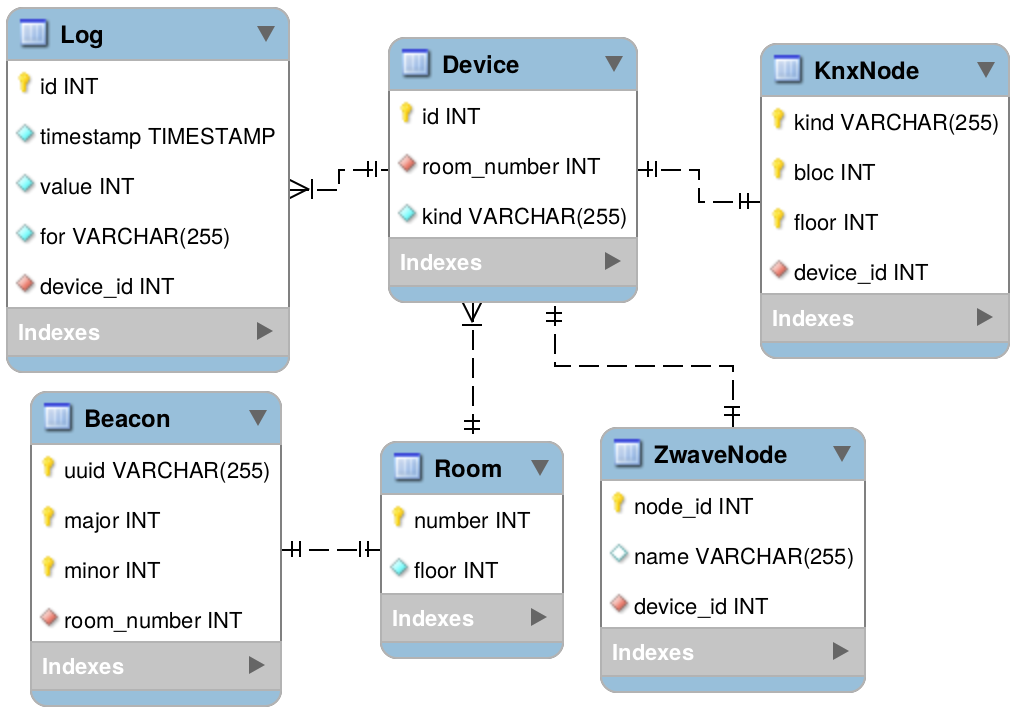
\includegraphics[width=0.8\textwidth]{img/diagramme_db.png}
    \end{center}
    \caption{Schéma relationnel de la base de données}
    \label{db_schema}
\end{figure}
